\documentclass[a4paper]{article}
\usepackage[utf8]{inputenc}
\usepackage[T1]{fontenc,url}
\usepackage[english,]{babel}
\usepackage{blindtext}
\usepackage{natbib}
\usepackage{gensymb}
\usepackage{amsmath}
\usepackage{amssymb}
\usepackage{commath}
\usepackage{physics}
\usepackage{multicol}
\usepackage{listings}
\usepackage{graphicx}
\usepackage{hyperref}
\usepackage{svg}
\usepackage{wrapfig}
\urlstyle{sf}



\newenvironment{Figure}
  {\par\medskip\noindent\minipage{\linewidth}}
  {\endminipage\par\medskip}

\def\doubleunderline#1{\underline{\underline{#1}}}
\makeatletter
\newcommand{\xRightarrow}[2][]{\ext@arrow 0359\Rightarrowfill@{#1}{#2}}
\makeatother

 
\usepackage{color}
 
\definecolor{codegreen}{rgb}{0,0.8,0.0}
\definecolor{codegray}{rgb}{0.5,0.5,0.5}
\definecolor{codepurple}{rgb}{0.28,0,0.82}
\definecolor{backcolour}{rgb}{0.95,0.95,0.92}
 
\lstdefinestyle{mystyle}{
    backgroundcolor=\color{backcolour},   
    commentstyle=\color{codegreen},
    keywordstyle=\color{magenta},
    numberstyle=\tiny\color{codegray},
    stringstyle=\color{codepurple},
    basicstyle=\footnotesize,
    breakatwhitespace=false,         
    breaklines=true,                 
    captionpos=b,                    
    keepspaces=true,                                    
    numbersep=5pt,                  
    showspaces=false,                
    showstringspaces=false,
    showtabs=false,                  
    tabsize=2
}
 
\lstset{style=mystyle}
 
\begin{document}
\vspace*{2cm}
\begin{center} 
 
\huge{Assignment 1}

\vspace{15mm}

\large{AST4320: Cosmology and Extragalatic Astronomy}

\vspace{5mm}

\normalsize{Metin San}

\vspace{5mm}

\normalsize{13. September 2018}

\vspace{25mm}

\end{center}

\newpage
\section*{Exercise 1}
\subsection*{(1)}

The continuity equation for an unperturbed universe driven by hubble expansion is given as 
\begin{equation}\label{eq:1}
\frac{d\bar{\rho}}{dt} + \bar{\rho} \nabla \cdot \mathbf{v}_0 = 0,
\end{equation}
where $\bar{\rho}$ is the average density of the universe, and $\mathbf{v}_0$ comes from the Hubble law today which states that 
\begin{equation}\label{eq:2}
\mathbf{v_0} = H_0 \mathbf{r}.
\end{equation}
Here $H_0$ is the Hubble parameter today, given as $H_0 = \dot{a}(t=t_0) / a(t = t_0)$, where $a$ is the scale factor, and is defined so that $a(t= t_0) = 1$. 

Inserting for \eqref{eq:2} into the continuity equation we find
\[
\frac{d\bar{\rho}}{dt} + \bar{\rho} \nabla \cdot \mathbf{r}  \frac{da}{dt} \frac{1}{a}= 0,
\]
where the del operator only works on $\mathbf{r}$ as its the scale factor is only a function of time. The operation results in $\nabla \cdot \mathbf{r} = 3$ which leaves us with
\[
\frac{d\bar{\rho}}{dt} + 3\bar{\rho}\frac{da}{dt} \frac{1}{a} = 0.
\]
We will then separate the equation
\[
\frac{d\bar{\rho}}{\rho} = -3 \frac{da}{a},
\]
where we also see that the $dt$ terms cancel each other out. This equation is then solved for the density by integrating both sides of the equation
\[
\int_{\bar{\rho}(t=t_0)}^{\bar{\rho}(t)} \frac{d\bar{\rho}}{\rho} = \int_{a(t=t_0)}^{a(t)} -3 \frac{da}{a},
\]
\[
\Rightarrow \ln \left( \frac{\bar{\rho}(t)}{\bar{\rho}(t=t_0)}\right) = \ln \left( \frac{a(t)}{a(t=t_0)}\right)^{-3}.
\]
This can then be reduced to
\begin{equation}\label{eq:3}
\bar{\rho}(t) = \bar{\rho}(t=t_0)a(t)^{-3},
\end{equation}
where we have used that $a(t=t_0) = 1$.


\subsection*{(2)}

The Poisson equation is given as
\begin{equation}\label{eq:4}
\nabla^2 \phi = 4 \pi G \rho.
\end{equation}
We will now study how small perturbations in quantities of interest evolve in time. We introduce the definition $\psi = \psi_0 +\delta \psi$, where $\psi$ is a variable of interest, $\psi_0$ is the unperturbed quantity and $\delta \psi$ is a little perturbation to that variable. The unperturbed Possion equation is then given as

\begin{equation}\label{eq:5}
\nabla^2 \phi_0 = 4 \pi G \rho_0.
\end{equation}
We can apply the perturbation definition to the gravitational potential $\phi$ and density $\rho$ in Poisson's equation, to get
\[
\nabla^2 (\phi_0 + \delta \phi) = 4\pi G (\rho_0 + \delta \rho)
\]
This can be written out on the form
\[
\nabla^2 \phi_0 + \nabla^2 \delta \phi = 4 \pi G \rho_0 +4 \pi G \delta \rho.
\]
We spot that the two terms $\nabla^2 \phi_0$ and $4 \pi G \rho_0$ equal the unperturbed Possion equation. These terms are then removed from the equation as they equal 0. This leaves us with the perturbed Poisson equation
\begin{equation}\label{eq:6}
\nabla^2 \delta \phi = 4 \pi G \delta \rho,
\end{equation}
Which describes how the perturbations evolve in time.
\\

A similar derivation can be carried out for the Euler equation. The equation of motion, or the Euler equation is given as
\begin{equation}\label{eq:7}
    \frac{d \mathbf{v}}{dt} = - \frac{1}{\rho} \nabla p - \nabla \phi.
\end{equation}
In terms of the perturbed quantities, this becomes
\[
    \frac{d (\mathbf{v_0} + \delta \mathbf{v})}{dt} = - \frac{1}{(\rho_0 + \delta \rho)} \nabla (p_0 + \delta p) - \nabla (\phi_0 + \delta \phi),
\]
where 
\begin{equation}\label{eq:8}
    \frac{d\mathbf{v_0}}{dt} = - \frac{1}{\rho_0} \nabla p_0  - \nabla \phi_0
\end{equation}
is the unperturbed equation.
Since the perturbed quantities are very small, we will make the approximation that $1/(\rho_0+ \delta \rho) \approx 1/\rho_0$. In addition to implementing this approximation, we also split up the RHS terms
\[
= - \frac{1}{\rho_0} \nabla p_0 - \frac{1}{\rho_0} \nabla \delta p - \nabla \phi_0 - \nabla \delta \phi.
\]
We spot that the two terms containing the perturbed quantities are equal the RHS of the unperturbed Euler equation \eqref{eq:8}, and we can replace them with $d\mathbf{v_0}/dt$, so that the RHS is simply
\[
= \frac{d\mathbf{v_0}}{dt} - \frac{1}{\rho_0} \nabla \delta p  - \nabla \delta \phi.
\]

We proceed with the LHS of the equation by writing out the total derivative

\[
 \frac{d (\mathbf{v_0} + \delta \mathbf{v})}{dt} = \frac{\partial (\mathbf{v_0} + \delta \mathbf{v})}{\partial t} + (\mathbf{v_0} + \delta \mathbf{v}) \cdot \nabla (\mathbf{v_0} + \delta \mathbf{v})
\]
\[
 = \frac{\partial \mathbf{v_0}}{\partial t} + \frac{\partial \delta \mathbf{v}}{\partial t} + \mathbf{v_0} \cdot \nabla \mathbf{v_0} + \delta \mathbf{v} \cdot \nabla \mathbf{v_0} + \mathbf{v_0}\cdot \nabla \delta \mathbf{v} + \delta \mathbf{v} \cdot \nabla \delta \mathbf{v}
\]
\[
= \frac{d \delta \mathbf{v}}{dt} + \frac{d \mathbf{v_0}}{dt} + \delta \mathbf{v} \cdot \nabla \mathbf{v}.
\]
In the last step we have used te fact that the the product of two infinitesimals are approximately 0. We have then rewritten back to total derivative form and gotten the extra $\delta \mathbf{v} \cdot \nabla \mathbf{v}$ term.

We can then collect both sides and cancel out the unperturbed terms, and we are left with the perturbed euler equation
\begin{equation}
    \frac{d \delta \mathbf{v}}{dt} + \delta \mathbf{v} \cdot \nabla \mathbf{v} = - \frac{1}{\rho_0} \nabla \delta p  - \nabla \delta \phi.
\end{equation}


\section*{Exercise 2}
\subsection*{(1)}
In the lectures, we sketched how one could arrive at the second order differential equation 

\begin{equation}
\frac{d^2 \delta}{dt^2} + 2 \frac{\dot{a}(t)}{a(t)} \frac{d \delta}{dt} = \delta(4 \pi G \rho_0 - k^2 c_s^2),
\end{equation}
which described the perturbation $\delta(t)$. Here $G$ is the gravitational constant, $k$ is the wavenumber of the perturbation given as $k = 2\pi/ \lambda$, and $c_s$ is the speed of sound in the medium.
≈

The Friedman equations can be used to derive the following expression for the Hubble rate or the time evolution of the scale factor 

\begin{equation}
\left(\frac{\dot{a}}{a}\right)^2 = H^2 = H_0^2 \left[ \frac{\Omega_m}{a^3} +  \Omega_\Lambda \right],
\end{equation}
where $\Omega_i$ is the fractional density parameter and
$i = m, \Lambda$ represents the matter and dark energy contributions to the density. We have assumed that the fractional radiation density is $\Omega_r = 0$. 

We will then specifically study the three scenarios where we have  $(\Omega_m, \Omega_\Lambda) = (1.0, 0.0)$, $(\Omega_m, \Omega_\Lambda) = (0.3, 0.7)$, and $(\Omega_m, \Omega_\Lambda) = (0.8, 0.2)$. 

Inserting these numbers into (11), we can find expressions for the $\dot{a}/a$ term for all three cases. Doing so gives us the following three expressions

\begin{equation}
\frac{\dot{a}}{a} = H_0 a^{-3/2}
\end{equation}

\begin{equation}
\frac{\dot{a}}{a} = H_0 \left[0.3a^{-3} + 0.7\right]^{1/2}
\end{equation}

\begin{equation}
\frac{\dot{a}}{a} = H_0  \left[0.8a^{-3} + 0.2\right]^{1/2}
\end{equation}
The first expression (12) corresponds to the Einstein-de Sitter Universe.

\subsection*{(2)}

We will now numerically solve differential equation (10). By using the critical density relation and assuming that perturbation is much larger than the Jeans length, we can rewrite the equation as
\begin{equation}
    \frac{d^2 \delta}{dt^2} + 2H\frac{d \delta}{dt} = \frac{3}{2}H^2 \delta,
\end{equation}
where it now only depends on $H$, which we previously derived.
In order to solve this numerically, we need to split the second order differential equation into two first order equations. We introduce the substitution 
\begin{equation}
    v = \frac{d\delta}{d t}.
\end{equation}
From this substitution it follows that
\begin{equation}
    \frac{dv}{dt} = \frac{3}{2}H^2 \delta - 2Hv.
\end{equation}

We will further use Euler's method to solve the differential equation iterative. One should in principle use methods of higher precision to avoid errors in the results, however, Euler's method seem to be sufficient in this case. In addition, our main interest lies in studying the behaviour of the perturbation and not necessarily the precise values. 

Euler's Method says that a general variable $y$ at a time $t + dt$ can be expressed as
\[
y(t + dt) = y(t) + \frac{dy}{dt} \cdot dt.
\]
Discretized, this can be written as 
\begin{equation}
    y_{i+1} = y_i + y_i'dt.
\end{equation}
By applying this method to our case, we end up with the following two equations we end up with the following set of equations

\begin{equation}
    v_{i+1} = v_i + \frac{dv}{dt}\cdot dt,
\end{equation}
\begin{equation}
    \delta_{i+1} = \delta_i + v_i.
\end{equation}
In order to simplify our lives, we also change variable from t to a, so that \[
dt = dt\frac{da}{da} = \frac{da}{\dot{a}},
\]
where $\dot{a} = H a$. 

We are given the boundary conditions $\log \delta = -3.0$ at $\log a = -3.0$. By assuming that $\delta \propto a$ at early times we find the initial condition of $\dot{\delta} \propto \dot{a}$. We are then ready to solve the differential equation for the three different universes. Doing so results in the following plot of the time evolution of the perturbations
\begin{figure}[h]
  \centering
  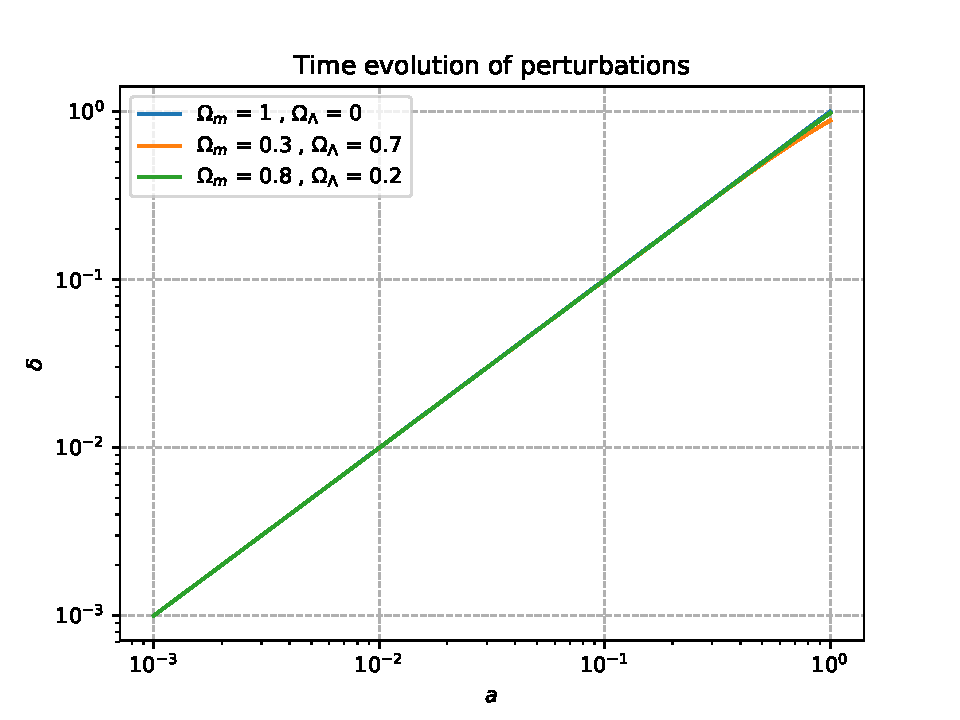
\includegraphics[width=0.9\linewidth]{2b.pdf}
  \caption{Time evolution of $\delta$ for the three different cosmologies with only matter and dark energy.}
  \label{fig:1}
\end{figure}

We see that for the Einstein-de Sitter case with $\Omega_m = 1$, the function is completely linear. This is expected as $\delta \propto a$ in this cosmology. For the two other cosmologies, we see that they also have a linear behaviour for most of the time scale. They do however begin to curve towards for higher values of a. This is because the matter term gets smaller as $a$ increases, and the cosmological constant begins to take over. 

\subsection*{(3)}
Having computed $\delta$ and $a$, we can now compute the growth factor $f$ given as 
\begin{equation}
    f \equiv \frac{d \ln \delta}{\ln a}.
\end{equation}
This is then plotted as a function of redshift z, where z is given as
\begin{equation}
    z +1 = \frac{a(t=t_0)}{a(t)}.
\end{equation}
Doing so results in the following plot 

\begin{figure}[h]
  \centering
  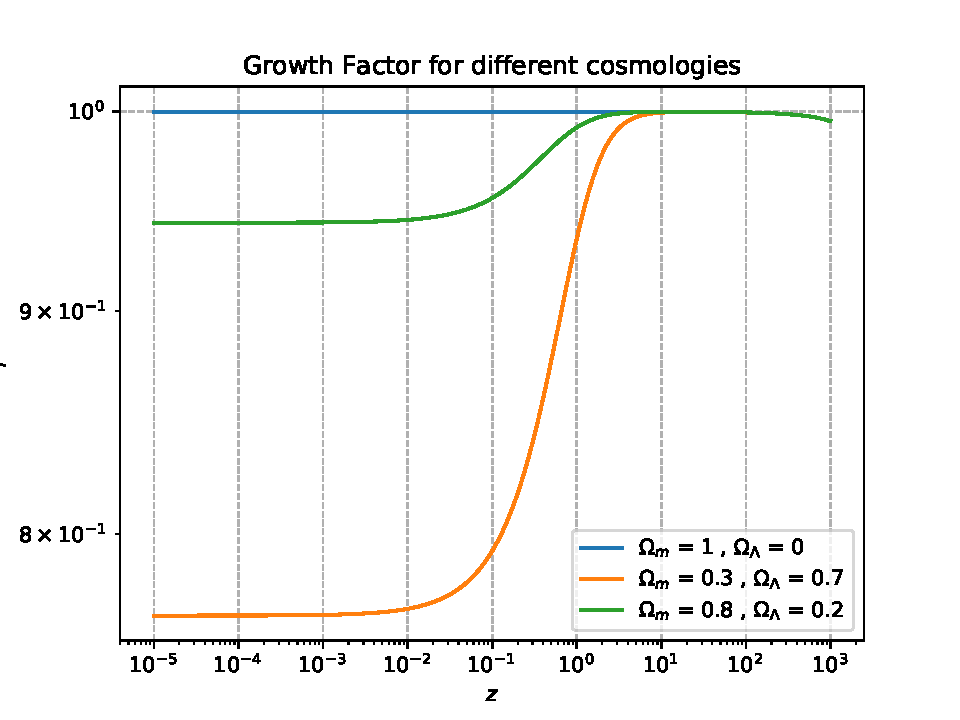
\includegraphics[width=0.9\linewidth]{growth.pdf}
  \caption{Growth factor for different cosmologies.}
  \label{fig:2}
\end{figure}
From figure \ref{fig:2} we see that the growth factor for the Einstein-de Sitter universe is basically constant at $f = 0$, meaning that there are no growth in this model. The two other models follows this flatness early in the history of the universe, but start to decrease when $z$ approaches $z =1$. We see again that the model with the largest $\Omega_\Lambda$ experiences the largest growth.

\section*{Exercise 3}

\subsection*{ (1) }

We will now study the temperature evolution of the radiation and gas in the universe in the range $a \in (10^{-4},1)$. We will assume that the both fluids evolve adiabatically though out the expansion of the universe. For an ideal gas whith adiabatic expansion, we have the following temperature volume relation

\begin{equation}
    TV^{\gamma-1} = C,
\end{equation}
where $\gamma$ is the degrees of freedom and $C$ is a constant. We assume that the universe is dominated by hydrogen, so that $\gamma = 5/3$ for an monatomic gas. Further we assume that the volume of the gas expands proportional to the expansion of the universe so that $V \propto a$. This leaves us with the following expression for the temperature of the gas

\begin{equation}
    T_\text{gas} = C a^{-2}.
\end{equation}


The considered radiation is the CMB radiation, which is a near perfect blackbody radiation. We can therfore use Wien's displacment law which says that the temperature of blackbody radiation is proportional to a constant divided by the wavelength
\begin{equation}
    T =  \frac{B}{\lambda}.
\end{equation}
$B$ is generally known, but we will use it as an unknown here and mainly focus on the fact that blackbody radiation is proportioanl to wavelength. We also know that the $\lambda \propto a$ because of redshift. This gives us the following relation for the temperature of the radiation
\begin{equation}
    T_\text{rad} = Ba^{-1}.
\end{equation}

In order to find the constant, we use the fact that the temperatures of the gas and radiation was the same during decoupling which occurred at $z = 1090$. At this time $T_\text{rad} = T_\text{gas} = 3000$K. Using this, we can solve equations (23) and (25) for $C$ and $B$. The results are then plotted and can be seen in figure (3).

\begin{figure}[h]
  \centering
  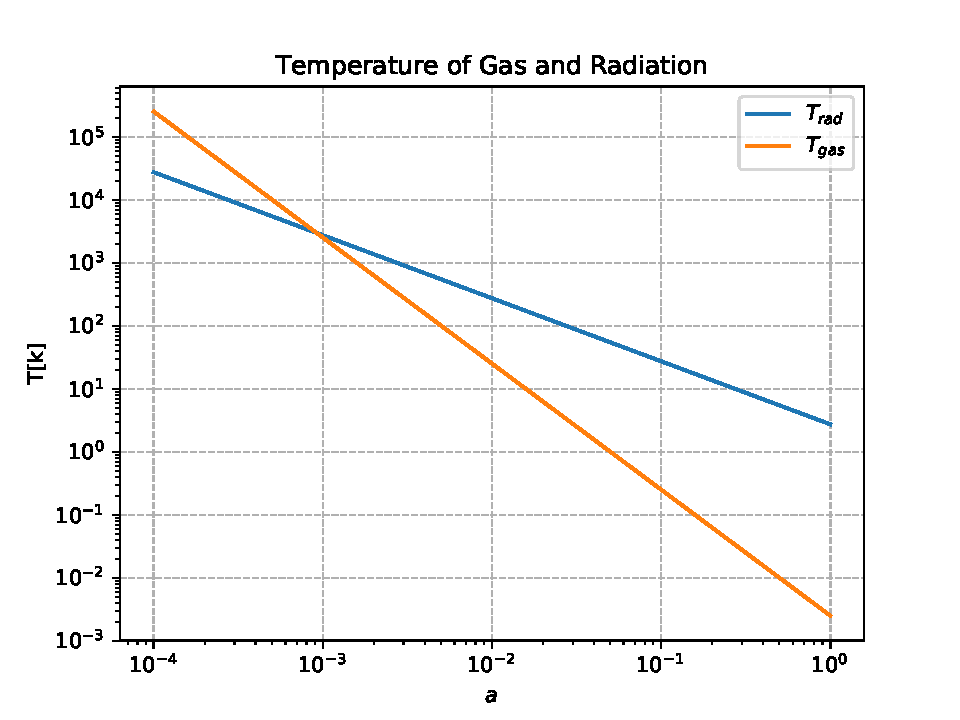
\includegraphics[width=0.9\linewidth]{Temp.pdf}
  \caption{Time evolution of gas and radiation temperature.}
  \label{fig:3}
\end{figure}

In reality both temperatures would have been equal until decoupling but our simple temperature mode does not account for this. We find that at $a = 1$ which is today, the temperature of the radiation is equal to $T(t=t_0) = 2.75$K. This is very close to the temperature of the CMB today which is $T_\text{CMB} = 2.725$. 

\subsection*{(2)}

We will now look at the Jeans length $\lambda_J$ and Jeans mass $M_J$. They are given as

\begin{equation}
    \lambda_J = c_s \sqrt{\frac{\pi}{G \rho}},
\end{equation}
\begin{equation}
    M_J = \frac{\pi^{5/2}}{6} \frac{c_s^3}{G^{3/2}\rho^{1/2}},
\end{equation}
where $c_s$ is the speed of sound and $G$ is the gravitational constant.
We are interested in finding out how they are related to redshift. We know that the speed of sound is given as

\begin{equation}
    c_s = \sqrt{\frac{k_B T}{\mu m_p}},
\end{equation}
where $k_B$ is the Boltzmann constant, $\mu$ is the average particle weight, and $m_p$ is the proton mass. We can now insert our the gas temperature found in the previous exercise. Doing so gives us
\begin{equation}
    c_s = \sqrt{\frac{k_B}{\mu m_p}} C^{1/2}a^{-1} = \sqrt{\frac{k_B C}{\mu m_p}}(1+z).
\end{equation}
We will also use the expression for density found in equation (3). Rewriting the Jeans mass and length in terms of these quantities, we end up with 

\begin{equation}
    \lambda_J = \sqrt{\frac{k_B \pi C }{\mu m_p G \rho_0}} (1+z)^{-1/2},
\end{equation}
\begin{equation}
    M_J =  \frac{\pi^{5/2}}{6 \rho^{1/2}}\left( \frac{k_B C}{\mu m_p G} \right)^{3/2} (1+z)^{3/2}.
\end{equation}
    
Prior to the decoupling, the plasma was relativistic, and the speed of sound was then a constant $c_s = c/ \sqrt{3}$ rather than a function of redshift.Using this expression to for the speed of sound, we find the following expressions for the Jeans length $\lambda'_J$ and mass $M'_J$ prior to decoupling

\begin{equation}
    \lambda'_J = \frac{c}{\sqrt{3}} \sqrt{\frac{\pi}{G\rho_0}}(1+z)^{-3/2},
\end{equation}
\begin{equation}
    M'_J = \frac{\pi^{5/2}}{6 G^{3/2}\rho_0^{1/2}} \frac{c^3}{(3)^{3/2}}(1+z)^{-3/2},
\end{equation}
where we see that the only redshift dependancy now comes from the density. We also spot that the pre decoupling expressions contain the speed of light $c$ which means that their amplitude will be much larger than the post decoupling expressions.

\section*{Exercise 4}

We will now consider the non-linear time-evolution of a spherical overdensity in the Einstein-de-Sitter Universe. We assume that this overdensity is confined into a sphere of radius $R(t) \equiv b(t)$, where $b(t)$ is the local scale factor. The acceleration of the radius of this sphere is then given by
\begin{equation}
    \ddot{R} = - \frac{GM}{R^2}.
\end{equation}
We will now show that the following parametrization 

\begin{align}
    R = A(1 - \cos \theta)\\
    t = B(\theta - \sin \theta)\\
    A^3 = GMB^2
\end{align}
satisfies the equation ($\ddot{R}$).

We start by inserting equation ($t$) solved for $B$ into ($A^3$), which gives us
\[
A^3 = \frac{GMt^2}{(\theta - \sin \theta)^2}.
\]
We can further insert this new expression for $A$ into equation ($R$) giving us the following equation for the radius of the sphere
\begin{equation}
    R(t) = \frac{(GM)^{1/3} (1- \cos \theta)}{(\theta - \sin \theta)^{2/3}} t^{2/3}.
\end{equation}
We will then use the first order Taylor approximations $\cos{\theta} \approx 1 - \theta^2/2! $ and $\sin{\theta} \approx \theta - \theta^3/3!$ . Inserting for these into equation $(R)$ we see that
\[
R(t) = \frac{(GM)^{1/3} \left(\frac{\theta^2}{2}\right)}{\left( \frac{\theta^3}{6}\right)^{2/3}} t^{2/3} = (GM)^{1/3}\left(\frac{6^{2/3}}{2}\right) t^{2/3}
\]
the expression becomes independent of the angles. We will now differentiate the angleless expression for the radius twice in order to find the acceleration. Doing so leave us with
\[
    \ddot{R} = - (GM)^{1/3} \left(\frac{6^{2/3}}{2}\right) \left(\frac{2}{9}\right) \frac{1}{t^{4/3}}.
\]
We will now multiply with $R(t)^2$ on both sides of the equation
\[
&   R^2 \ddot{R} = - (GM)^{1/3} \left(\frac{6^{2/3}}{2}\right)               \left(\frac{2}{9}\right) \frac{1}{t^{4/3}} \cdot             (GM)^{2/3}\left(\frac{6^{2/3}}{2}\right)^2 t^{4/3}.
\]
We see that the constant numbers cancel each other, and we are simply left with
\[
R^2 \ddot{R}=  - GM.
\]
By dividing both sides with $R^2$, we end up with the desired results
\begin{equation*}
    \ddot{R} = - \frac{GM}{R^2},
\end{equation*}
which means that the parametrization is satisfied.

\section*{Exercise 5}

We will now compute the infall velocity $v$ from when the material in the overdensity first reaches the viral radius $R_{\text{vir}}$. We will do so by using the parametrization in exercise 4. The infall velocity is given as
\[
    v = \frac{dR}{dt},
\]
where $R$ is the radius from equation (15). By using the chain rule, we can express this as 
\[
    \frac{dR}{dt} = \frac{dR}{d\theta} \frac{d \theta}{dt}.
\]
We start by computing $dR/d\theta$ by differentiating equation (15) with respect to $\theta$
\[
    \frac{dR}{d\theta} = \frac{d}{d\theta} A(1-\cos\theta) = A \sin \theta.
\]
Similarly, we compute $d\theta/dt$ by differentiating expression (16) with respect to $\theta$
\[
    \frac{dt}{d\theta} = \frac{d}{d\theta} B(\theta-\sin\theta) = B(1 - \cos \theta).
\]
and then inverting it. Combining these terms gives us
\[
    v = \frac{A \sin \theta}{B (1- \cos \theta)}.
\]
If we now square each side of the equation, we get
\[
v^2 = \frac{A^2 \sin^2 \theta}{B^2 (1-\cos \theta)^2}.
\]
Further we solve equation (18) for $B^2$ and substitute in
\[
v^2 = \frac{GM\sin^2 \theta}{A(1-\cos \theta)^2}
\]
and then insert for equation (15) solved for $A$, which gives us
\[
    v^2 = \frac{GM \sin^2 \theta}{R (1-\cos \theta)}.
\]
We know that radius equals the virialization radius $R=R_\text{vir}$ when $\theta = 3\pi / 2$. We plug in the virialization angle and find
\[
    v^2 = \frac{GM}{R_\text{vir}}.
\]
Finally, by taking the square root on both sides, we find the following equation for the infall velocity

\begin{equation}
    v = \sqrt{\frac{GM}{R_\text{vir}}}.
\end{equation}
\section*{Exercise 6}

We can derive the gravitational binding energy of a uniform sphere of radius $R$ and mass $M$ by assuming that the density within the sphere i constant. The density is then given as the total mass divided by the volume of the sphere
\[
\rho = \frac{M}{\frac{4}{3} \pi R^3}.
\]
We then assume that the sphere is divided into thin layers or shells with the mass of the outermost shell being
\[
m_{\text{shell}} = 4\pi R^2 \rho\, dR.
\]
The remaining mass within the volume of the outer shell is then
\[
m_{\text{interior}} = \frac{4}{3}\pi R^3 \rho.
\]
The energy required for the outer shell to escape the gravitational pull is then given as
\[
dU = -G\frac{m_{\text{shell}} m_{\text{interior}} }{R}.
\]
We find the total energy by inserting for the masses and integrating over all shells
\[
U = -G \int^R_0 \frac{\left(4\pi R^2 \rho\right)  \left(\frac{4}{3}\pi R^3 \rho \right)}{R} dR
\]
\[
= - \frac{16}{3} G\pi^2 \rho^2 \int_0^R R^4 dR
\]
Solving the integral leaves us with 
\[
U = - \frac{16}{15} G \pi^2 \rho^2 R^5.
\]
Finally by inserting for the density, we get

\[
U = - \frac{16}{15} G \pi^2 R^5 \left(\frac{M}{\frac{4}{3} \pi R^3}\right)^2 = - \frac{3}{5} \frac{GM^2}{R},
\]
which was to be shown.
\end{document}